\documentclass[
  scale = 1.5,
]{hftpostr}

\title{Bachelor Thesis: Entwicklung eines deflektometrischen Prüfaufbaus für spiegelnde Prüfobjekte}
\author{Vipin Singh}
\advisor{Prof. Dr.-Ing. Uwe Müßigmann}

\usetheme{PosterHFT1}
\usepackage{wrapfig}
\usepackage[format=hang]{caption}
\usepackage[export]{adjustbox}
\usepackage{pgfkeys}
\usepackage{tikz}
\usepackage{tkz-euclide}
\usepackage{pgfplots}
\pgfplotsset{compat=1.18}
\usetikzlibrary{shapes.callouts,shapes.geometric,calc,positioning,decorations.markings}
\graphicspath{{./poster_bilder/}} %Bilder

\begin{document}

\begin{frame}[t]
\vspace{-0.75\baselineskip}
	\begin{block}{Motivation}
		Die optischen Besonderheiten von glänzenden Oberflächen faszinieren zahlreiche Menschen.
		Bereits Neugeborene fühlen sich den Reflexionen von Glanzobjekten hingezogen.
		Auch die industriellen Bereiche wollen diese Faszination der Leute ansprechen.
		So befinden sich an vielen Stellen im Alltag glänzende Oberflächen, um Menschen zu begeistern.
		Die riesige Menge an produzierten Bauteilen und die hohen Qualitätsanforderungen machen eine automatisierte Prüfung der Teile unumgänglich.
		Dabei stoßen die üblichen Verfahren der industriellen Bildverarbeitung auf ihre Grenzen, sodass neue Methoden eingeführt werden müssen.
		Diese speziellen Anwendungen erfordern den Einsatz von deflektometrischen Prüfaufbauten, die sich die Spiegelung von bestimmten Szenen zunutze machen.
	\end{block}
	
	\vskip -2.5ex
	
	\begin{columns}[onlytextwidth, T]
		\begin{column}{.71\textwidth}
			\begin{block}{Problematik}
				\begin{wrapfigure}{r}{0.58\textwidth}
					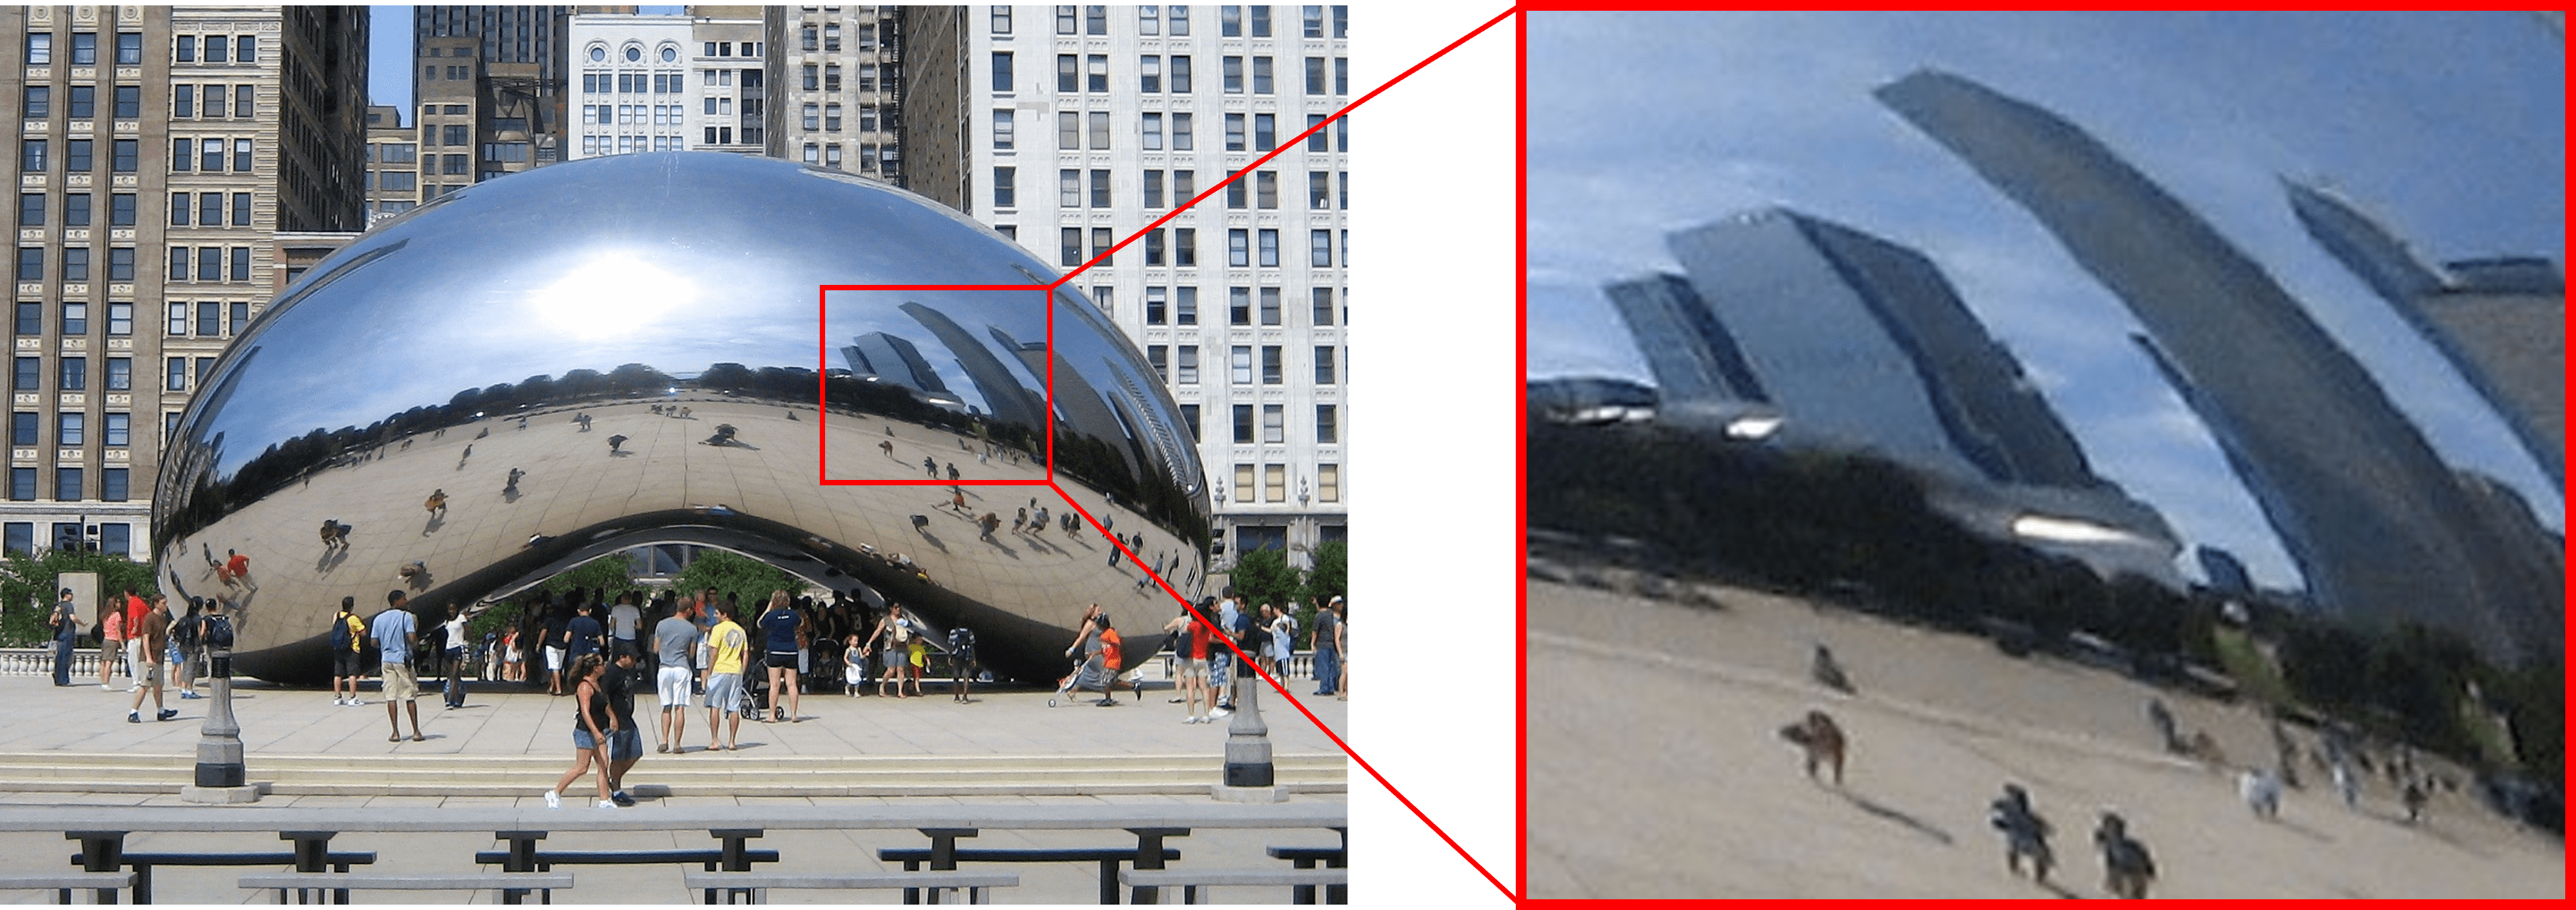
\includegraphics[width=0.56\textwidth]{cloudGateMitAusschnitt}
					\caption{Cloud Gate aus Chicago mit Spieglung von Gebäuden}
				\end{wrapfigure}
				Die Schwierigkeit besteht darin, dass beim Betrachten einer spiegelnden Oberfläche stets ein verzerrtes Bild der Umgebung zu sehen ist.
				Allein aus diesen verzerrten Szenen, wie z. B. auf dem Ausschnitt aus der rechten Abbildung, sollen Informationen zur Oberflächenbeschaffenheit gewonnen werden.
			\end{block}
		\end{column}
		
		\begin{column}{0.25\textwidth}
			\begin{block}{Deflektometrie}
				Die Deflektometrie bezeichnet Methoden zur optischen Erfassung von Gestaltinformationen spiegelnder Oberflächen durch Auswertung von Spiegelbildern bekannter Szenen.
				Als Szenen werden meistens Muster über einen Bildschirm auf die Oberfläche abgebildet.
			\end{block}
		\end{column}
	\end{columns}
	
	\begin{columns}[onlytextwidth, T]
		\begin{column}{.48\textwidth}
			\begin{block}{Verfahren 1: Sichtprüfung durch Lichtstreuung}
				\begin{wrapfigure}{l}{0.52\textwidth}
						
\includegraphics[width=0.5\textwidth]{aufbau}
						\caption{Aufbau des Verfahrens für transparente Prüfobjekte}
				\end{wrapfigure}

				Dieses Verfahren wurde optimiert für spiegelnde transparente Prüfobjekte und nutzt die abweichende Lichtstreuung bzw. Lichtbrechung an Oberflächendefekten.
				Trifft Licht auf einen lokalen Defekt, so wird das Licht abweichend von der Umgebung des Defekts in verschiedene Richtungen gestreut.
				Es werden Streifenmuster auf dem Bildschirm hinter dem transparenten Objekt angezeigt und die Kamerabilder durch geeignete Bildarithmetik verknüpft.
				Als Ergebnis erhält man Bilder, in denen Oberflächenanomalien wie z. B. Kratzer oder Gravuren sichtbar werden.
				
				\begin{wrapfigure}{l}{0.35\textwidth}
					\vspace{-0.5\baselineskip}
					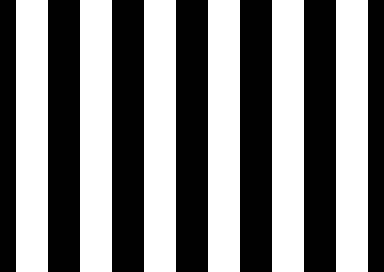
\includegraphics[frame,width=0.33\textwidth]{rechteckMuster}
					\caption{Streifenmuster}
				\end{wrapfigure}
				
				\par\bigskip
				Sequenzen von Streifenmustern wie in der linken Abbildung können nach diesem Verfahren verwendet werden, um Kratzer und Gravuren auf Brillengläsern zu erfassen. (siehe Abbildung unten)
				
				\begin{figure}
					\vspace{3\baselineskip}
					\centering
					\begin{tikzpicture}[every node/.style={inner sep=0,outer sep=0}]
	
						\node [anchor=north east] (img1) at (-0.05\textwidth,0) {\includegraphics[width=.45\textwidth]{gefärbtesBrillenglas2_rotiert_Bild}};
						\node [anchor=north west] (img2) at (0.05\textwidth,0) {\includegraphics[width=.45\textwidth]{gefärbtesBrillenglas2_rotiert_verbessert_Norm_LookUp}};
						
						\draw[very thick,-{Latex[width=3mm]},shorten >=0.02\textwidth,shorten <=0.02\textwidth] (img1.east) -- (img2.west);
						
					\end{tikzpicture}
					\caption{Hervorhebung von Kratzern und Gravuren auf einem Brillenglas}
				\end{figure}
				\vspace{-0.75\baselineskip}
			\end{block}
		\end{column}
		
		\begin{column}{.48\textwidth}
			\begin{block}{Verfahren 2: Deflektometrische Registrierung}
				\begin{wrapfigure}{r}{0.63\textwidth}
						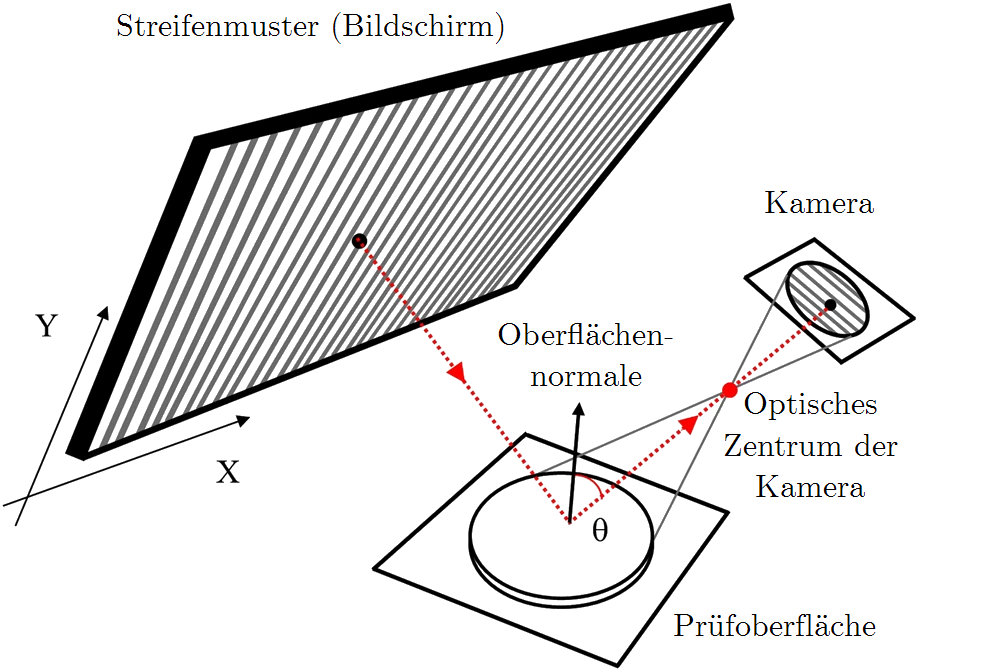
\includegraphics[width=0.61\textwidth]{output-onlinepngtools}
						\caption{Aufbau des Verfahrens für spiegelnde Prüfobjekte}
				\end{wrapfigure}
				Dieses Verfahren wurde speziell für spiegelnde nicht-transparente Objekte entwickelt, auf denen man Spiegelbilder der Szenen ohne störende Reflexionen gut erkennen kann.
				Es werden die Ortskoordinaten des Bildschirms bzw. der Szene durch bestimmte Muster kodiert (z. B. über Grauwerte).
				Die verzerrten Spiegelbilder der Szenen werden schließlich dekodiert, um die Ortskoordinaten im Kamerabild zuzuordnen.
				Die Zuordnung wird deflektometrische Registrierung genannt und kann weiterverarbeitet werden, um Krümmungsinformationen der Oberfläche zu erhalten.
				
				\begin{wrapfigure}{r}{0.35\textwidth}
					\vspace{-0.5\baselineskip}
					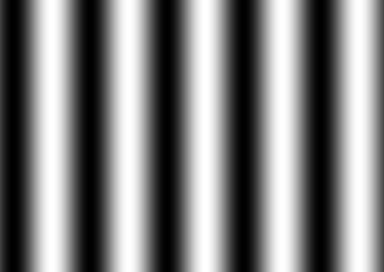
\includegraphics[frame,width=0.33\textwidth]{phasenMuster}
					\caption{Streifenmuster}
					\vspace{\baselineskip}
				\end{wrapfigure}
				
				\par\bigskip
				Zur Bestimmung der deflektometrischen Registrierung können Sequenzen von sinusoidalen Streifenmustern (siehe Abbildung rechts) zur Kodierung verwendet werden. 
				Dadurch wird es möglich, Defekte, wie z. B. Dellen oder Oberflächenpickel auf spiegelnden Oberflächen zu erfassen. (siehe Abbildung unten)
				
				\begin{figure}
					\centering
					\begin{tikzpicture}[every node/.style={inner sep=0,outer sep=0}]
	
						\node [anchor=north east] (img1) at (-0.05\textwidth,0) {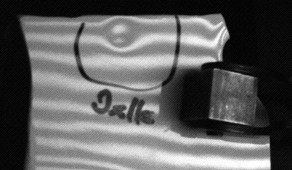
\includegraphics[width=.45\textwidth]{keramikobjekt_2_streifenmuster}};
						\node [anchor=north west] (img2) at (0.05\textwidth,0) {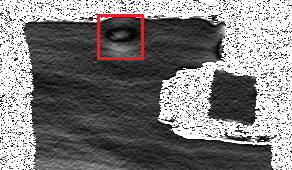
\includegraphics[width=.45\textwidth]{keramikobjekt_2_ableitung}};
						
						\draw[very thick,-{Latex[width=3mm]},shorten >=0.02\textwidth,shorten <=0.02\textwidth] (img1.east) -- (img2.west);
						
					\end{tikzpicture}
					\caption{Hervorhebung einer Delle auf einem spiegelnden Keramikobjekt}
				\end{figure}
				\vspace{-0.75\baselineskip}
			\end{block}
		\end{column}
	\end{columns}	
	
\end{frame}
\end{document}